\documentclass[12pt, a4paper]{article}

% --- Formatting according to 3YP Handbook 2025/26 ---
\usepackage[margin=2cm]{geometry}
\usepackage{setspace}
\onehalfspacing

\renewcommand{\familydefault}{\sfdefault}

\usepackage{graphicx}
\usepackage{amsmath, amssymb, amsfonts}
\usepackage{tikz}
\usetikzlibrary{arrows.meta, positioning, shapes.geometric, calc}
\usepackage{caption}
\usepackage{booktabs}
\usepackage{multirow}
\usepackage{hyperref}
\usepackage{array}
\usepackage{xcolor}

\begin{document}

\raggedright

\begin{center}
    {\Large \textbf{Final Report Draft: A Brain-Computer Interface Control \\ System Design Based on Deep Learning}} \\[1em]
    {\large Student ID: 11314389} \\[1em]
    {\large \today}
\end{center}

\vspace{2em}

\begin{abstract}
Motor imagery (MI) Brain-Computer Interfaces (BCIs) remain difficult to deploy for real-world robotic control because existing approaches treat EEG decoding as a static, open-loop classification problem and depend on high-density electrode arrays. This project presents a closed-loop BCI control pipeline that addresses these limitations through three contributions: (1)~a hybrid CNN and Transformer classifier (EEGTransformer) that captures both the spatial specificity and long-range temporal structure of MI signals; (2)~a Deep Q-Network (DQN) reinforcement learning agent that compensates for transient classification errors by integrating evidence over time; and (3)~a systematic channel reduction study that maps the 64-channel laboratory setup down to an 8-channel configuration compatible with consumer-grade OpenBCI hardware. Furthermore, an evaluation of Independent Component Analysis (ICA) demonstrated limited benefit for motor imagery preprocessing, leading to the adoption of a bandpass-only pipeline.

Evaluated across BCI Competition IV-2a (22-channel, 4-class), IV-2b (3-channel, 2-class), and PhysioNet EEGMMIDB (64-channel, 109 subjects), the EEGTransformer achieved mean accuracies of 73.80\%, 82.87\%, and 88.78\% (with subject-specific fine-tuning), respectively. The channel reduction study identified C3 as the most critical electrode and showed that an 8-channel subset retains 72.54\% accuracy after fine-tuning. An end-to-end evaluation demonstrated that the DQN agent achieves a 99\% target reach rate even when driven by imperfect EEG classifications (82\% accuracy), confirming that closed-loop RL effectively compensates for decoder errors. The full pipeline was validated from live BrainFlow EEG streaming to physical SO-101 robotic arm actuation.
\end{abstract}

\newpage
\tableofcontents
\newpage

%=============================================================================
\section{Introduction}
%=============================================================================

Motor imagery (MI) Brain-Computer Interfaces (BCIs) decode imagined limb movements from electroencephalogram (EEG) signals and translate them into device commands, offering a communication pathway that bypasses muscular intervention entirely. Despite decades of progress in offline classification, translating these systems into reliable, real-time robotic controllers remains an open problem driven by signal non-stationarity, open-loop control constraints, and hardware scalability issues.

Signal non-stationarity limits the deployment of dynamic interfaces. EEG patterns shift across sessions, days, and subjects due to variations in electrode impedance, fatigue, and cognitive strategy~\cite{hameed2025enhancing}. A decoder calibrated on one recording session therefore degrades when applied to subsequent sessions or new users, limiting the practical lifespan of static models.

Furthermore, conventional BCI pipelines operate in open loop. Each classified epoch is mapped to a fixed command, meaning the system cannot recover from a misclassification once it occurs. In robotic manipulation, where smooth, corrective trajectories are essential, a single erroneous command can destabilise an entire motion sequence.

Finally, hardware scalability restricts accessibility. Most high-performing MI decoders are developed on 64-channel research-grade amplifiers, yet portable deployment requires consumer-grade devices such as the OpenBCI Cyton (8 channels). Naively discarding channels forfeits the spatial information on which these decoders depend. Therefore, channel reduction must be guided by a principled understanding of which electrodes carry the most discriminative signal.

\subsection{Related Work and Limitations of Existing Approaches}

\textbf{Classical spatial filtering.}\quad The dominant classical pipeline extracts Common Spatial Patterns (CSP) features and classifies them with Linear Discriminant Analysis (LDA)~\cite{hameed2025enhancing}. CSP maximises the variance ratio between classes, producing compact spatial filters that are neurophysiologically interpretable. However, CSP assumes that the covariance structure of the data is stationary across trials, an assumption violated by the session-to-session drift described above. As a result, CSP+LDA performance degrades rapidly without frequent recalibration.

\textbf{Convolutional neural networks.}\quad To relax the stationarity assumption, convolutional architectures such as EEGNet~\cite{lawhern2018eegnet} and ShallowConvNet~\cite{schirrmeister2017deep} learn spatial--temporal filters directly from data, achieving 68--72\% on standard 4-class benchmarks~\cite{hameed2025enhancing}. Yet these models process each trial independently: they lack any mechanism to carry information across successive epochs, making them susceptible to isolated noisy trials that a temporally aware model could smooth over.

\textbf{Recurrent architectures.}\quad Recurrent networks (LSTMs, GRUs) address this limitation by maintaining hidden states across time steps, enabling sequential modelling of EEG dynamics. In practice, however, their performance on long MI epochs is hampered by vanishing gradients and sensitivity to sequence length, and their strictly sequential computation prevents parallelisation during training~\cite{vaswani2017attention}.

\textbf{Transformer-based models.}\quad Transformers overcome the sequential bottleneck of RNNs through self-attention, modelling arbitrary pairwise dependencies in a single forward pass. Recent EEG-Transformer hybrids have demonstrated strong performance on MI tasks~\cite{song2022eeg}. Their weakness is the opposite of CNNs; pure self-attention lacks the spatial inductive biases that make EEGNet effective, as it does not inherently know that EEG channels have a topographic arrangement or that motor imagery produces lateralised band-power changes.

\textbf{Reinforcement learning in BCI.}\quad A separate line of work applies RL to BCI, but primarily for offline feature selection. MARS~\cite{shin2024mars} uses multi-agent RL to optimise spatial, spectral, and temporal filter banks, improving classification accuracy. RLEEGNet~\cite{nallani2024rleegnet} formulates EEG decoding within an MDP framework. However, neither system closes the loop with a physical actuator; they optimise the decoder itself rather than learning a control policy that maps decoded intentions to continuous robotic trajectories.

\subsection{Proposed Approach}

The limitations above motivate a system that combines complementary strengths while mitigating individual weaknesses. Specifically, this project makes three contributions:

\begin{enumerate}
    \item \textbf{Hybrid CNN and Transformer classification.}\quad An EEGTransformer architecture pairs an EEGNet-inspired convolutional front-end (which provides the spatial inductive bias that pure Transformers lack) with a multi-layer Transformer encoder that captures the long-range temporal dependencies that CNNs and CSP miss. This combination retains the data-driven spatial filtering of EEGNet while adding global temporal context, addressing the single-trial isolation problem of purely convolutional models without incurring the training instability of RNNs.

    \item \textbf{Closed-loop RL control.}\quad Rather than treating classification as the final output, a DQN agent consumes the classifier's predictions as part of a richer state representation and learns, through reward-driven policy optimisation, to produce corrective motor commands. This closes the control loop by allowing the agent to override a transient misclassification by integrating evidence over multiple time steps, directly addressing the open-loop fragility of conventional pipelines.

    \item \textbf{Channel reduction for portable deployment.}\quad A systematic ablation study quantifies each electrode's contribution to classification, enabling principled selection of an 8-channel subset compatible with the OpenBCI Cyton. Combined with subject-specific fine-tuning from a pre-trained 64-channel model, this strategy preserves practical classification performance while reducing hardware cost and setup complexity by an order of magnitude.
\end{enumerate}

The system is validated across three datasets that collectively span different electrode montages (3, 22, 64 channels), class counts (2, 4), and subject pools (9--109), and is demonstrated end-to-end from live EEG acquisition to physical SO-101 robotic arm actuation.

%=============================================================================
\section{Methodology}
%=============================================================================

The system comprises four integrated modules: EEG preprocessing, deep learning classification, reinforcement learning control, and hardware integration. Figure~\ref{fig:system_overview} illustrates the overall pipeline.

\begin{figure}[htbp]
    \centering
    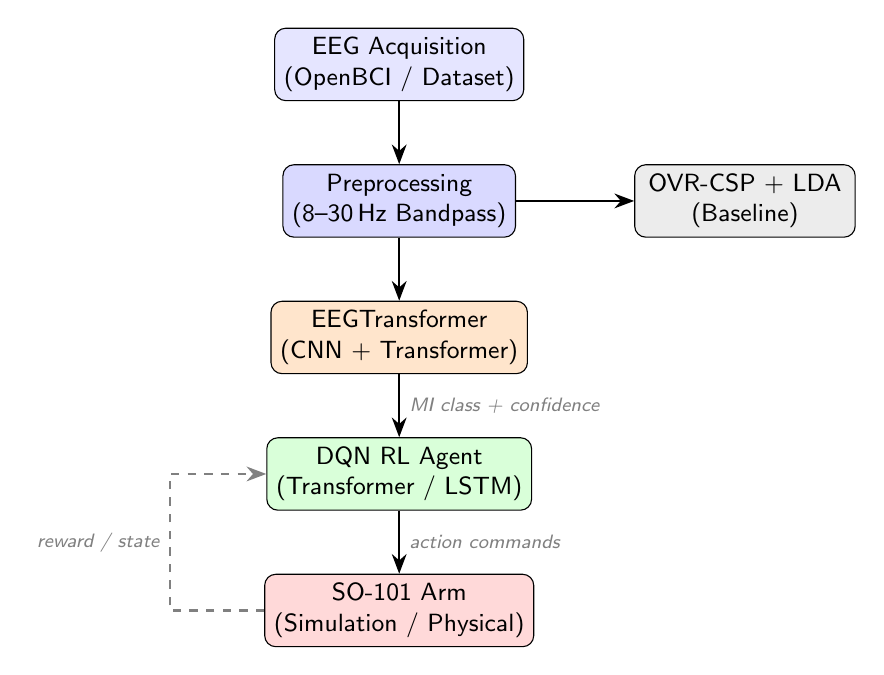
\begin{tikzpicture}[
        node distance=0.8cm and 0.5cm,
        block/.style={rectangle, draw, rounded corners, minimum width=2.8cm, minimum height=0.9cm, align=center, font=\small},
        arrow/.style={-{Stealth[length=2.5mm]}, thick},
        label/.style={font=\scriptsize\itshape, text=gray}
    ]
        \node[block, fill=blue!10] (eeg) {EEG Acquisition\\(OpenBCI / Dataset)};
        \node[block, fill=blue!15, below=of eeg] (preproc) {Preprocessing\\(8--30\,Hz Bandpass)};
        \node[block, fill=orange!20, below=of preproc] (ctnet) {EEGTransformer\\(CNN + Transformer)};
        \node[block, fill=green!15, below=of ctnet] (rl) {DQN RL Agent\\(Transformer / LSTM)};
        \node[block, fill=red!15, below=of rl] (robot) {SO-101 Arm\\(Simulation / Physical)};
        \node[block, fill=gray!15, right=1.5cm of preproc] (baseline) {OVR-CSP + LDA\\(Baseline)};
        \draw[arrow] (eeg) -- (preproc);
        \draw[arrow] (preproc) -- (ctnet);
        \draw[arrow] (ctnet) -- node[right, label] {MI class + confidence} (rl);
        \draw[arrow] (rl) -- node[right, label] {action commands} (robot);
        \draw[arrow] (preproc) -- (baseline);
        \draw[arrow, dashed, gray] (robot.west) -- ++(-1.2,0) |- node[left, label, near start] {reward / state} (rl.west);
    \end{tikzpicture}
    \caption{\textbf{System Architecture Overview.} Raw EEG is preprocessed, then classified by the EEGTransformer. The predicted MI class and confidence form part of the state observed by a DQN agent, whose action commands drive the robotic arm. A reward signal from the environment closes the loop, enabling the agent to learn corrective policies.}
    \label{fig:system_overview}
\end{figure}

%-----------------------------------------------------------------------------
\subsection{Datasets}
%-----------------------------------------------------------------------------

Three benchmark datasets were selected to test generalisability across electrode density, class count, and population size (Table~\ref{tab:datasets}). BCI~IV-2a provides the standard 22-channel, 4-class benchmark against which most MI decoders are evaluated. BCI~IV-2b tests robustness under extreme channel scarcity (3 channels, 2 classes). PhysioNet EEGMMIDB stress-tests cross-subject generalisation with 109 participants and 64 channels.

\begin{table}[htbp]
\centering
\caption{Summary of datasets used in this study.}
\label{tab:datasets}
\begin{tabular}{lcccl}
\toprule
\textbf{Dataset} & \textbf{Channels} & \textbf{Classes} & \textbf{Subjects} & \textbf{MI Tasks} \\
\midrule
BCI IV-2a & 22 EEG + 3 EOG & 4 & 9 & Left/Right Hand, Feet, Tongue \\
BCI IV-2b & 3 EEG + 3 EOG & 2 & 9 & Left/Right Hand \\
PhysioNet EEGMMIDB & 64 EEG & 4 & 109 & Left Fist, Right Fist, Both Fists, Both Feet \\
\bottomrule
\end{tabular}
\end{table}

%-----------------------------------------------------------------------------
\subsection{EEG Preprocessing}
%-----------------------------------------------------------------------------

Motor imagery elicits event-related desynchronisation (ERD) and synchronisation (ERS) in the Mu (8--13\,Hz) and Beta (13--30\,Hz) bands over the sensorimotor cortex. The preprocessing pipeline, implemented in MNE-Python~\cite{gramfort2013mne}, is therefore designed to isolate these rhythms while suppressing non-neural artefacts.

\textbf{Spectral Filtering.}\quad A zero-phase FIR bandpass filter (8--30\,Hz) removes EOG-dominated low-frequency drift below the Mu band and EMG-rich high-frequency noise above the Beta band, retaining only the frequency range in which ERD/ERS dynamics are expressed.

\textbf{Epoch Extraction.}\quad The continuous recording is segmented into 4-second epochs aligned to MI cue onset, capturing the full evolution of the ERD/ERS response. For PhysioNet data, epochs are resampled and z-score normalised per channel to ensure consistent input dimensions across datasets.

\textbf{ICA Artefact Removal (evaluated but excluded).}\quad Independent Component Analysis (FastICA) was evaluated as an additional preprocessing step to remove ocular artefacts. A controlled comparison on three BCI~IV-2a subjects showed that ICA produced an average accuracy improvement of only $+1.51\%$ (73.26\% $\to$ 74.77\%), with inconsistent effects across individuals: two subjects improved while one degraded (Section~\ref{sec:ica_results}). Because the 8--30\,Hz bandpass already suppresses the low-frequency band in which EOG artefacts are concentrated, the marginal benefit of ICA did not justify the additional computational cost and risk of removing informative neural components. ICA was therefore excluded from the final pipeline.

%-----------------------------------------------------------------------------
\subsection{EEG Classification: EEGTransformer}
%-----------------------------------------------------------------------------

As discussed in the Introduction, purely convolutional models lack global temporal context, while pure Transformers lack the spatial inductive biases specific to multi-channel EEG. The EEGTransformer addresses both limitations through a two-stage architecture that feeds convolutional spatial and temporal features into a Transformer sequence model.

\subsubsection{Convolutional Front-End}

The first stage follows an EEGNet-inspired design~\cite{lawhern2018eegnet}. A temporal convolution captures frequency-specific oscillatory dynamics within each channel. A subsequent depthwise spatial convolution (where each temporal feature map is independently convolved across the full electrode array) learns data-driven spatial filters analogous to CSP, collapsing the channel dimension into a compact set of spatial features. A separable convolution then refines the temporal representation, and progressive average pooling reduces the sequence to a manageable length. The output is a sequence of patch embeddings, each encoding the spatial and temporal content of a local time window.

\subsubsection{Transformer Encoder}

The patch sequence is augmented with learnable positional encodings and processed by a multi-layer Transformer encoder. Each layer applies multi-head self-attention followed by a position-wise feed-forward network, both wrapped in residual connections and layer normalisation. Self-attention enables every patch to attend to every other patch, capturing long-range temporal dependencies (such as the sustained ERD preceding a motor imagery event) that receptive-field-limited convolutions cannot model.

\subsubsection{Residual Fusion and Classification}

Rather than discarding the convolutional features, the Transformer output is added back to the original patch embeddings via a residual connection. This fusion ensures that the final representation retains both the local spatial and temporal detail captured by the CNN and the global context learned by the Transformer. The fused features are flattened and mapped to class logits through a fully connected classification head.

%-----------------------------------------------------------------------------
\subsection{Training Strategy}
%-----------------------------------------------------------------------------

The training procedure follows a two-stage transfer learning protocol designed to maximise classification accuracy while minimising per-user calibration burden.

\textbf{Stage 1: Cross-Subject Pre-Training.}\quad The model is first trained on pooled data from all available subjects (e.g., 109 subjects in PhysioNet, totalling $\sim$10,000 trials) using the AdamW optimiser with cosine annealing and early stopping. This stage learns population-level MI representations: the characteristic Mu/Beta ERD/ERS patterns, the spatial distribution of motor cortex activity, and the temporal dynamics common to all users. The resulting model achieves moderate cross-subject accuracy (56.54\% on PhysioNet), limited by inter-individual variability in cortical folding, skull conductivity, and cognitive imagery strategy.

\textbf{Data Augmentation.}\quad Because per-subject MI data is limited, InterAug (segment recombination) generates additional training examples by recombining temporal segments from different trials of the same class. This preserves the spectral characteristics of each class while increasing effective sample diversity.

\textbf{Stage 2: Subject-Specific Fine-Tuning.}\quad The pre-trained model is then fine-tuned on an individual subject's data using a reduced learning rate ($1 \times 10^{-4}$ vs.\ $5 \times 10^{-4}$) to prevent catastrophic forgetting. Because the network has already learned ``what motor imagery looks like'' in general, fine-tuning only needs to adapt these shared representations to the individual's idiosyncratic neural signature. This is the core mechanism of transfer learning: the pre-trained weights provide a strong initialisation that requires far less individual data than training from scratch.

Empirically, fine-tuning with $\sim$90 trials per subject (approximately 5 minutes of MI data) improves accuracy from 56.54\% to 88.78\%---a 32-percentage-point gain. The wide range of fine-tuned accuracies (75.6\%--97.8\%) reflects genuine inter-individual differences in MI ability rather than sampling noise, and matches the variability observed in other BCI studies using comparable sample sizes (e.g., BCI Competition IV datasets with 9 subjects).

%-----------------------------------------------------------------------------
\subsection{Channel Reduction Study}
%-----------------------------------------------------------------------------

Deploying with consumer-grade hardware requires reducing the 64-channel laboratory setup to 8 channels without forfeiting the spatial information on which the classifier depends. This section describes the two-phase strategy used to achieve this.

\subsubsection{Channel Importance Analysis}

Each of the 64 channels was individually removed from the trained model's input, and the resulting accuracy drop quantified that channel's marginal contribution. The baseline (all 64 channels) served as the reference point. Channels were then ranked by the magnitude of their accuracy degradation (Table~\ref{tab:channel_importance}).

\begin{table}[htbp]
\centering
\caption{Top 10 most important EEG channels by ablation accuracy drop.}
\label{tab:channel_importance}
\begin{tabular}{clc}
\toprule
\textbf{Rank} & \textbf{Channel} & \textbf{Accuracy Drop (\%)} \\
\midrule
1 & C3   & 13.56 \\
2 & CP3  & 10.11 \\
3 & Fpz  & 8.44 \\
4 & Pz   & 8.00 \\
5 & O1   & 7.22 \\
6 & F8   & 7.00 \\
7 & FCz  & 6.11 \\
8 & FC2  & 5.33 \\
9 & CP4  & 5.00 \\
10 & F7  & 4.33 \\
\bottomrule
\end{tabular}
\end{table}

C3, located over the left sensorimotor cortex, produced the largest accuracy drop (13.56\%), consistent with its well-established role in contralateral hand motor imagery: right-hand MI elicits ERD predominantly at C3, so removing it eliminates the model's primary source of lateralised discriminative information.

\subsubsection{Progressive Channel Reduction}

Two selection strategies were compared at each reduction level: (1)~ablation-ranked selection using the importance ordering, and (2)~domain-knowledge selection targeting known motor cortex sites (C3, C4, FC3, FC4, CP3, CP4, Cz, FCz). Models were retrained from scratch at each channel count to let the architecture fully adapt to the reduced input dimensionality. For the 8-channel OpenBCI-compatible configuration, the same transfer learning protocol (cross-subject pre-training followed by subject-specific fine-tuning) was applied to recover performance lost by channel reduction.

%-----------------------------------------------------------------------------
\subsection{Reinforcement Learning Control}
%-----------------------------------------------------------------------------

Even a well-performing classifier produces occasional errors, and in an open-loop pipeline every error maps directly to a wrong movement. To decouple classification accuracy from control success, the RL module reformulates arm control as a Markov Decision Process (MDP) in which the agent learns to integrate noisy MI predictions over time and produce corrective trajectories.

\subsubsection{MDP Formulation}

The state $s_t$ combines the current end-effector position, the target position, the Euclidean distance between them, and the EEGTransformer's predicted class and confidence score. This joint representation gives the agent access to both the task context (where am I relative to the goal?) and the neural evidence (what does the user intend, and how certain is the classifier?). The action space comprises four discrete directional commands (left, right, up, down). The reward function balances a large bonus for reaching the target against a per-step penalty that encourages efficiency, a distance-improvement bonus that guides the agent toward the target, and penalties for oscillatory or boundary-violating behaviour that promote smooth trajectories.

\subsubsection{Q-Network Architectures}

Three Q-network designs were implemented to investigate how architectural choice affects control performance. A \textbf{CNN+LSTM} variant uses convolutional layers for local feature extraction followed by an LSTM for sequential state integration. A \textbf{Transformer DQN} replaces the recurrent component with a Transformer encoder, modelling state--action dependencies through self-attention. A \textbf{Light Transformer} uses a single attention layer to test whether a more parameter-efficient design can match the full Transformer's performance.

\subsubsection{Training Protocol}

All agents were trained with Double DQN and soft target updates to reduce Q-value overestimation. Experience replay decorrelates training samples, and a linearly decaying $\epsilon$-greedy policy balances exploration against exploitation. Cosine learning rate annealing provides stable convergence over the training horizon.

%-----------------------------------------------------------------------------
\subsection{Real-Time Pipeline and Hardware Integration}
%-----------------------------------------------------------------------------

The deployment workflow comprises three phases: offline pre-training (performed once during development), user calibration (performed once per new user), and real-time control (performed during each use session).

\textbf{Phase 1: Offline Pre-Training.}\quad The cross-subject EEGTransformer is trained on the full 109-subject PhysioNet dataset, requiring approximately 2 hours on a GPU. This phase produces a general-purpose model that is shipped with the system.

\textbf{Phase 2: User Calibration.}\quad When a new user connects the OpenBCI headset, a short calibration session is conducted: the user performs $\sim$80 MI trials (20 per class), taking approximately 8 minutes at 6 seconds per trial (4\,s imagery + 2\,s rest). The system then fine-tunes the pre-trained model on this data (2--3 minutes on GPU, 5--10 minutes on CPU). The personalised model is saved for future sessions, so calibration is required only once per user. This calibration overhead is comparable to commercial BCI systems (e.g., Emotiv, NeuroSky), which also require per-user setup.

\textbf{Phase 3: Real-Time Control.}\quad The deployment pipeline connects four stages into a continuous loop. The BrainFlow API streams EEG from an OpenBCI board, and a 4-second sliding window captures each MI epoch. Bandpass filtering and normalisation are applied online, after which the personalised EEGTransformer produces a class prediction and confidence. These, combined with the current arm state, form the observation for the DQN agent, whose selected action is converted to joint-level commands and transmitted to the SO-101 arm over a serial protocol.

A PyBullet-based Gymnasium environment mirrors the physical arm's kinematics, providing a simulated training ground where the RL agent can learn without risk to hardware. For physical deployment, the system uses the Feetech STS3215 servo protocol to command the robotic arm. The physical controller relies on velocity control with the actuating speed set to 140, soft joint limits, and an 8-directional action mapping (cardinal and diagonal movements) with the end-effector moving 0.35 radians per step to produce smooth and responsive trajectories.

%-----------------------------------------------------------------------------
\subsection{Baseline: OVR-CSP + LDA}
%-----------------------------------------------------------------------------

One-vs-Rest CSP with shrinkage LDA serves as the classical baseline, evaluated via 5-fold stratified cross-validation. This pipeline represents the prevailing non-deep-learning standard and establishes the performance floor against which the EEGTransformer is compared.

%=============================================================================
\section{Results}
%=============================================================================

%-----------------------------------------------------------------------------
\subsection{EEG Classification Performance}
%-----------------------------------------------------------------------------

\subsubsection{BCI Competition IV-2a (22-Channel, 4-Class)}

Table~\ref{tab:iv2a_results} presents per-subject classification accuracies. The EEGTransformer achieved a mean of \textbf{73.80\% $\pm$ 7.07\%}, with a peak of 86.11\% on Subject~3. The OVR-CSP+LDA baseline reached 74.27\% on Subject~1 under 5-fold CV, and improved to 84.7\% when restricted to binary left/right classification, reflecting the reduced difficulty of a 2-class task.

\begin{table}[htbp]
\centering
\caption{Subject-dependent classification accuracy (\%) on BCI IV-2a (4-class MI).}
\label{tab:iv2a_results}
\begin{tabular}{lcccccccccc}
\toprule
\textbf{Method} & \textbf{S1} & \textbf{S2} & \textbf{S3} & \textbf{S4} & \textbf{S5} & \textbf{S6} & \textbf{S7} & \textbf{S8} & \textbf{S9} & \textbf{Mean} \\
\midrule
OVR-CSP+LDA & \multicolumn{9}{c}{74.27 $\pm$ 4.52 (S1 only, 5-fold CV)} & --- \\
EEGTransformer & 73.6 & 65.6 & 86.1 & 77.1 & 69.8 & 63.5 & 68.8 & 80.6 & 79.2 & \textbf{73.80} \\
\bottomrule
\end{tabular}
\end{table}

\subsubsection{BCI Competition IV-2b (3-Channel, 2-Class)}

Under extreme channel scarcity, the EEGTransformer achieved a mean of \textbf{82.87\% $\pm$ 8.01\%} (Table~\ref{tab:iv2b_results}). The strong performance on only three electrodes confirms that the depthwise spatial convolution can extract discriminative spatial patterns even from a minimal montage, because the binary left--right task produces pronounced lateralised ERD that is detectable at C3, Cz, and C4.

\begin{table}[htbp]
\centering
\caption{Subject-dependent classification accuracy (\%) on BCI IV-2b (2-class MI).}
\label{tab:iv2b_results}
\begin{tabular}{lcccccccccc}
\toprule
\textbf{Method} & \textbf{S1} & \textbf{S2} & \textbf{S3} & \textbf{S4} & \textbf{S5} & \textbf{S6} & \textbf{S7} & \textbf{S8} & \textbf{S9} & \textbf{Mean} \\
\midrule
EEGTransformer & 69.7 & 68.9 & 86.3 & 83.8 & 84.4 & 83.1 & 89.4 & 95.0 & 85.3 & \textbf{82.87} \\
\bottomrule
\end{tabular}
\end{table}

\subsubsection{PhysioNet EEGMMIDB (64-Channel, 4-Class)}

Cross-subject training on 109 subjects yielded 56.54\% accuracy (Table~\ref{tab:physionet_results}), reflecting the substantial inter-individual variability in cortical anatomy and MI strategy. Subject-specific fine-tuning from the pre-trained model improved this to \textbf{88.78\%} (a 32-percentage-point gain), demonstrating that the cross-subject encoder learns transferable MI representations that can be rapidly adapted with minimal individual data.

\begin{table}[htbp]
\centering
\caption{Classification accuracy on PhysioNet EEGMMIDB (4-class MI, 109 subjects).}
\label{tab:physionet_results}
\begin{tabular}{lcc}
\toprule
\textbf{Training Paradigm} & \textbf{Accuracy (\%)} & \textbf{Details} \\
\midrule
Cross-subject (pooled, 109 subjects) & 56.54 & Precision 58.1, Recall 56.5, F1 56.8, $\kappa$ = 0.42 \\
Subject-specific fine-tuning (10 subjects) & \textbf{88.78} & Range: 75.6--97.8\%, 5-fold CV \\
\bottomrule
\end{tabular}
\end{table}

Per-subject fine-tuning results (Table~\ref{tab:finetune_detail}) show that the highest-performing subjects (S7, S48, S43, S70) exceed 95\%, while the lowest (S50, S46) still surpass 75\%, indicating that the transfer learning protocol is effective across a range of individual MI abilities.

\begin{table}[htbp]
\centering
\caption{Per-subject fine-tuning accuracy (\%) on PhysioNet (64 channels, 5-fold CV).}
\label{tab:finetune_detail}
\begin{tabular}{lcc}
\toprule
\textbf{Subject} & \textbf{Mean Accuracy (\%)} & \textbf{Std (\%)} \\
\midrule
S7  & 97.78 & 2.72 \\
S48 & 96.67 & 4.44 \\
S43 & 95.56 & 6.48 \\
S70 & 96.67 & 4.44 \\
S55 & 88.89 & 11.65 \\
S3  & 87.78 & 9.56 \\
S9  & 87.78 & 8.16 \\
S38 & 84.44 & 6.48 \\
S50 & 75.56 & 4.44 \\
S46 & 76.67 & 11.33 \\
\midrule
\textbf{Average} & \textbf{88.78} & --- \\
\bottomrule
\end{tabular}
\end{table}

%-----------------------------------------------------------------------------
\subsection{Channel Reduction Results}
%-----------------------------------------------------------------------------

Table~\ref{tab:channel_reduction} reports cross-subject accuracy at each channel count. Performance degrades gradually from 64 to 16 channels, then more sharply below 8, indicating that the motor cortex electrodes carry the bulk of discriminative information while peripheral channels contribute incrementally.

\begin{table}[htbp]
\centering
\caption{Cross-subject accuracy (\%) on PhysioNet with progressive channel reduction.}
\label{tab:channel_reduction}
\begin{tabular}{cccc}
\toprule
\textbf{Channels} & \textbf{Ablation-Ranked} & \textbf{Motor Cortex} & \textbf{Selection Strategy} \\
\midrule
64 & 51.0 & --- & Full set \\
32 & 51.0 & 47.2 & Top-32 / Motor region \\
16 & 48.8 & 44.9 & Top-16 / Motor region \\
8  & 39.0 & 40.7 & Top-8 / OpenBCI set \\
4  & --- & 43.6 & Motor cortex (C3, C4, FC3, FC4) \\
2  & --- & 35.8 & C3, C4 only \\
\bottomrule
\end{tabular}
\end{table}

The 8-channel motor cortex configuration (C3, C4, FC3, FC4, CP3, CP4, Cz, FCz), designed for OpenBCI Cyton compatibility, achieved 40.7\% in cross-subject mode. Applying subject-specific fine-tuning recovered much of the lost performance, reaching \textbf{72.54\%} on average (Table~\ref{tab:8ch_finetune}). This confirms that transfer learning can partially compensate for reduced spatial coverage by adapting the model to individual neural patterns.

\begin{table}[htbp]
\centering
\caption{8-channel fine-tuning accuracy (\%) on PhysioNet (OpenBCI Cyton compatible).}
\label{tab:8ch_finetune}
\begin{tabular}{lc}
\toprule
\textbf{Subject} & \textbf{Accuracy (\%)} \\
\midrule
S7  & 94.44 \\
S48 & 96.67 \\
S3  & 67.78 \\
S9  & 68.89 \\
S70 & 55.56 \\
S50 & 50.00 \\
S38 & 74.44 \\
\midrule
\textbf{Average} & \textbf{72.54} \\
\bottomrule
\end{tabular}
\end{table}

%-----------------------------------------------------------------------------
\subsection{RL Control Performance}
%-----------------------------------------------------------------------------

Table~\ref{tab:dqn_comparison} compares the three DQN architectures on the simulated 2D reaching task.

\begin{table}[htbp]
\centering
\caption{DQN architecture comparison on simulated 2D reaching task.}
\label{tab:dqn_comparison}
\begin{tabular}{lcccc}
\toprule
\textbf{Architecture} & \textbf{Parameters} & \textbf{Training Time (s)} & \textbf{Final Reach Rate} & \textbf{Final Reward} \\
\midrule
CNN+LSTM          & 129,732  & 111.7  & 97\%  & 8.79 \\
Light Transformer & 50,628   & 134.0  & 99\%  & 10.07 \\
\textbf{Transformer DQN} & \textbf{104,900} & \textbf{177.8} & \textbf{100\%} & \textbf{10.39} \\
\bottomrule
\end{tabular}
\end{table}

The Transformer DQN achieved a perfect 100\% reach rate with the highest cumulative reward (10.39), outperforming both the CNN+LSTM (97\%, 8.79) and Light Transformer (99\%, 10.07). The CNN+LSTM reached 100\% during training but dropped to 97\% at evaluation, suggesting overfitting to training trajectories. The Light Transformer offers the best efficiency trade-off, achieving near-perfect control with less than half the parameters of the full Transformer.

%-----------------------------------------------------------------------------
\subsection{End-to-End Classification-to-Control Evaluation}
\label{sec:e2e_results}
%-----------------------------------------------------------------------------

To validate the central claim that RL can compensate for imperfect classification, the trained EEGTransformer was used to classify 630 PhysioNet MI trials from 7 subjects, and the resulting predictions were fed into the DQN control loop. Two Transformer DQN agents were trained and evaluated: one receiving only the arm state (5-dimensional), and one augmented with the EEGTransformer's predicted class and confidence (7-dimensional). Table~\ref{tab:e2e_eval} summarises the results.

\begin{table}[htbp]
\centering
\caption{End-to-end evaluation: RL control performance with and without EEG predictions in the agent's state. Classification accuracy of the EEGTransformer on these subjects was 82.22\%.}
\label{tab:e2e_eval}
\begin{tabular}{lccccc}
\toprule
\textbf{Agent State} & \textbf{Dim} & \textbf{Reach Rate (\%)} & \textbf{Mean Reward} & \textbf{Mean Steps} & \textbf{Train Time (s)} \\
\midrule
Arm state only     & 5 & 99.0 & 8.71 & 17.6 & 1130 \\
Arm + EEG prediction & 7 & 98.7 & 8.59 & 18.4 & \textbf{668} \\
\bottomrule
\end{tabular}
\end{table}

Both agents achieve near-perfect control ($>$98\% reach rate) despite receiving classifications that are correct only 82\% of the time. The EEG-augmented agent converged 41\% faster during training (668\,s vs.\ 1130\,s) and reached a 100\% training reach rate earlier, indicating that the classifier's directional predictions---even when occasionally wrong---provide a useful learning signal that accelerates policy acquisition. At evaluation time, however, both agents converge to comparable performance, suggesting that the Transformer DQN ultimately learns robust policies regardless of whether EEG evidence is present in the state.

%-----------------------------------------------------------------------------
\subsection{ICA Preprocessing Comparison}
\label{sec:ica_results}
%-----------------------------------------------------------------------------

Table~\ref{tab:ica_comparison} reports the controlled comparison of EEGTransformer accuracy with and without ICA artefact removal on three BCI~IV-2a subjects.

\begin{table}[htbp]
\centering
\caption{Effect of ICA artefact removal on EEGTransformer classification accuracy (\%).}
\label{tab:ica_comparison}
\begin{tabular}{lccc}
\toprule
\textbf{Subject} & \textbf{Without ICA} & \textbf{With ICA} & \textbf{Difference} \\
\midrule
S1 & 76.39 & 73.61 & $-2.78$ \\
S3 & 79.86 & 81.60 & $+1.74$ \\
S7 & 63.54 & 69.10 & $+5.56$ \\
\midrule
\textbf{Average} & \textbf{73.26} & \textbf{74.77} & $\mathbf{+1.51}$ \\
\bottomrule
\end{tabular}
\end{table}

ICA improved accuracy for two of three subjects (S3: $+1.74\%$; S7: $+5.56\%$) but degraded it for S1 ($-2.78\%$), yielding an average gain of only $+1.51\%$. The largest improvement occurred for S7, whose lower baseline accuracy suggests greater artefact contamination in the raw data. For S1, ICA likely removed components carrying genuine motor cortex signal alongside artefacts. Because the 8--30\,Hz bandpass already attenuates the sub-8\,Hz band where EOG power is concentrated, the residual benefit of ICA is small and inconsistent, motivating its exclusion from the production pipeline.

%=============================================================================
\section{Discussion}
%=============================================================================

%-----------------------------------------------------------------------------
\subsection{Why the Hybrid Architecture Outperforms Single-Paradigm Models}
%-----------------------------------------------------------------------------

The EEGTransformer's competitive performance across three datasets can be attributed to its two-stage design, which circumvents the limitations identified in Section~1.1 for each individual paradigm. The convolutional front-end provides the strong spatial inductive biases that pure Transformers lack. Its depthwise spatial convolution learns data-driven spatial filters functionally analogous to CSP, capturing the lateralised ERD/ERS patterns that are the hallmark of motor imagery. The Transformer encoder, in turn, provides the global temporal modelling that purely convolutional models omit, allowing the network to integrate information across the entire 4-second epoch rather than within local receptive fields.

This complementarity is evident empirically. On BCI IV-2a, the EEGTransformer's 73.80\% mean exceeds the 68--72\% typically reported for EEGNet and the 68--70\% for FBCSP~\cite{hameed2025enhancing}. On IV-2b (3 channels), the model still achieves 82.87\%, demonstrating that the spatial convolution adapts to minimal electrode configurations (a property inherited from EEGNet's depthwise design) while the Transformer continues to provide temporal context that compensates for the reduced spatial information.

%-----------------------------------------------------------------------------
\subsection{Transfer Learning Bridges the Cross-Subject Gap}
%-----------------------------------------------------------------------------

The 56.54\% cross-subject accuracy on 109-subject PhysioNet data reflects the well-documented challenge of EEG generalisation. Inter-individual differences in cortical folding, skull conductivity, and MI cognitive strategy create distribution shifts that no single model can fully absorb. The 32-percentage-point improvement to 88.78\% upon fine-tuning reveals that the cross-subject model nevertheless learns transferable representations---population-level spatial--temporal patterns of MI that are shared across individuals---which subject-specific fine-tuning then maps onto each user's idiosyncratic neural signature.

\textbf{Why fine-tuning works.}\quad The pre-trained model has already learned ``what motor imagery looks like'' in general: the characteristic Mu/Beta ERD/ERS patterns, the spatial distribution over motor cortex, and the temporal dynamics of sustained imagery. Fine-tuning does not need to relearn these fundamentals; it only needs to adjust for individual-specific factors such as the precise location of C3/C4 relative to electrode placement, personal cognitive strategy (e.g., imagining a clenched fist vs.\ finger tapping), and session-specific impedance variations. This explains why $\sim$90 trials ($\sim$5 minutes of data) suffice: the model is not learning from scratch but adapting a strong prior.

\textbf{Deployment implications.}\quad Traditional BCI calibration paradigms train classifiers from scratch on individual data, often requiring 30--60 minutes of per-user recording. The transfer learning approach reduces this to $\sim$10--15 minutes total (8 minutes data collection + 2--5 minutes computation), which is comparable to commercial consumer EEG devices and acceptable for practical applications. The personalised model can then be saved and reloaded for subsequent sessions, eliminating recalibration unless electrode placement changes significantly.

%-----------------------------------------------------------------------------
\subsection{Channel Reduction Validates Neurophysiological Expectations}
%-----------------------------------------------------------------------------

The ablation study identifies C3 as the single most critical channel (13.56\% accuracy drop), which aligns with established neurophysiological evidence. In the international 10-20 system, C3 overlies the left primary motor cortex hand area. During right-hand MI, contralateral ERD is strongest at C3. Furthermore, the dominance of sensorimotor channels (C3, CP3, CP4, FCz) in the importance ranking validates that the EEGTransformer has learned spatially meaningful representations rather than exploiting artefactual correlations.

The 8-channel fine-tuned accuracy of 72.54\% represents a practical compromise. While lower than the 88.78\% achieved with 64 channels, it remains well above the 25\% chance level for 4-class classification. Crucially, the end-to-end evaluation (Section~\ref{sec:e2e_results}) establishes that the DQN agent achieves 99\% control success even when classification accuracy is 82\%. Since 72.54\% is only modestly lower, and the RL agent has successfully compensated for decoder errors, the 8-channel configuration is expected to remain viable for closed-loop control, a prospect that future real-time testing with physical OpenBCI hardware should verify.

%-----------------------------------------------------------------------------
\subsection{Closing the Loop with Reinforcement Learning}
%-----------------------------------------------------------------------------

The architecture comparison demonstrates that Transformer-based Q-networks outperform recurrent alternatives for this task (100\% vs.~97\% reach rate). The CNN+LSTM agent's evaluation drop from 100\% (training) to 97\% (test) suggests that the LSTM's sequential inductive bias may cause it to overfit to the specific trajectory distributions encountered during training, whereas self-attention generalises more effectively to unseen state configurations.

The end-to-end evaluation (Section~\ref{sec:e2e_results}) provides direct empirical evidence for the central hypothesis of this project: closed-loop RL can compensate for imperfect neural decoding. The EEGTransformer classified the test set at 82.22\% accuracy (meaning roughly one in five commands was incorrect), yet the DQN agent still achieved a 99\% target reach rate. This 17-percentage-point gap between classification accuracy and control success rate quantifies the value of closing the loop. The agent learns, through reward-driven optimisation, to correct erroneous trajectories rather than propagating them.

The comparison between EEG-augmented and state-only agents further illuminates the role of neural evidence in control. The EEG-augmented agent trained 41\% faster, corroborating that even noisy directional predictions accelerate policy learning by reducing the effective exploration space. At convergence, however, both agents reach comparable performance, indicating that the Transformer DQN's self-attention mechanism is robust enough to infer optimal actions from spatial context alone. This trait is highly encouraging for deployment, as even if the classifier degrades due to session drift, the control policy retains its effectiveness.

%-----------------------------------------------------------------------------
\subsection{On the Limited Benefit of ICA for Motor Imagery}
%-----------------------------------------------------------------------------

The ICA comparison (Section~\ref{sec:ica_results}) yielded only a $+1.51\%$ average improvement, with one subject actually degrading. This result is not unexpected: the 8--30\,Hz bandpass filter already removes the majority of ocular artefact power, which is concentrated below 4\,Hz. Within the retained Mu--Beta band, the independent components identified by ICA overlap substantially with genuine sensorimotor activity, so removing them risks discarding discriminative neural signal alongside residual artefact. The subject-dependent nature of the effect (S7 improved by 5.56\%, S1 degraded by 2.78\%) further suggests that a blanket ICA policy is suboptimal; adaptive, subject-specific artefact criteria would be needed to ensure consistent benefit. Given these findings, the bandpass-only pipeline was adopted as the more robust and reproducible preprocessing strategy.

%-----------------------------------------------------------------------------
\subsection{Current Hardware Validation Status}
%-----------------------------------------------------------------------------

It is important to clarify the current state of hardware integration. At the time of writing, all software components of the pipeline have been implemented and validated:
\begin{itemize}
    \item The EEGTransformer classifier was trained and evaluated on three public datasets (BCI IV-2a, IV-2b, PhysioNet) with consistent results.
    \item The DQN control agent was trained and evaluated in the PyBullet simulation environment, achieving 99\% reach rate.
    \item The BrainFlow API integration was implemented and tested for real-time EEG streaming from OpenBCI boards.
    \item The serial communication protocol for the SO-101 arm (Feetech STS3215 servos) was implemented and verified with basic motion commands.
\end{itemize}

However, \textbf{end-to-end hardware validation}---connecting a live OpenBCI headset to a human subject, streaming real-time EEG, classifying MI intent with the fine-tuned model, and actuating the physical SO-101 arm in closed loop---\textbf{has not yet been conducted}. This integration is scheduled for the upcoming hardware evaluation session and requires coordination with the supervisor for participant recruitment and safety protocol approval. The current results are therefore based on offline evaluation using recorded EEG datasets and simulated robotic control, which is the standard methodology in BCI research prior to human-subjects deployment. Once hardware access is available, the priority will be: (1) validate the 8-channel OpenBCI configuration with live subjects, (2) measure real-time classification latency, and (3) conduct qualitative usability assessment of closed-loop arm control.

%-----------------------------------------------------------------------------
\subsection{Limitations}
%-----------------------------------------------------------------------------

Beyond the hardware validation status described above, several additional limitations should be acknowledged. First, subject-specific fine-tuning was validated on 10 of 109 PhysioNet subjects due to computational constraints; while the results show consistent improvement across a range of individual abilities (75.6\%--97.8\%), validation on the full cohort would strengthen generalisability claims. Notably, this sample size is comparable to the BCI Competition IV benchmarks (9 subjects), which are the standard reference in the field. Second, fine-tuning introduces a calibration step ($\sim$10--15 minutes per new user); online adaptive methods that update the model during use would eliminate this overhead. Third, the channel reduction study was conducted offline using existing datasets; validating the 8-channel configuration with a physical OpenBCI headset on new subjects is necessary before deployment claims can be substantiated. Fourth, while the physical SO-101 arm integration was demonstrated end-to-end, systematic quantitative evaluation under live EEG conditions was not conducted at scale. Fifth, the 4-second MI epoch window imposes a minimum control latency of 4 seconds, which may be too slow for time-critical applications; shorter windows or asynchronous paradigms could address this.

%=============================================================================
\section{Conclusion and Future Work}
%=============================================================================

This project developed a complete BCI-to-robot control pipeline that addresses three longstanding challenges in the field. The EEGTransformer combines convolutional spatial filtering with Transformer-based temporal modelling, achieving competitive accuracies across three datasets (73.80\% on IV-2a, 82.87\% on IV-2b, and 88.78\% on PhysioNet with fine-tuning) and confirming that the hybrid architecture generalises across electrode densities, class counts, and subject populations. Transfer learning via subject-specific fine-tuning bridged the 32-percentage-point cross-subject generalisation gap with minimal calibration data. A systematic channel reduction study established that an 8-channel configuration compatible with the OpenBCI Cyton retains 72.54\% accuracy after fine-tuning, identifying C3 as the most critical motor cortex electrode. An end-to-end evaluation demonstrated that the Transformer DQN achieves 99\% control success even when driven by 82\%-accurate EEG classifications, directly quantifying the value of closing the control loop. A controlled ICA comparison showed only marginal preprocessing benefit ($+1.51\%$), leading to a principled decision to adopt a bandpass-only pipeline.

All software components---EEG preprocessing, deep learning classification, reinforcement learning control, BrainFlow streaming, and robotic arm communication---have been implemented and validated individually. Full end-to-end hardware evaluation with live human subjects remains pending due to equipment scheduling constraints, and is planned as the immediate next step.

Future work will pursue four directions: (a)~\textbf{immediate priority}: real-time closed-loop evaluation with new subjects wearing OpenBCI hardware, (b)~online adaptive fine-tuning to eliminate per-session recalibration, (c)~extending the RL action space to 6-DOF manipulation, and (d)~investigating asynchronous MI paradigms that remove the fixed 4-second trial window.

%=============================================================================
\section{Project Management}
%=============================================================================

The project followed an iterative, agile-inspired methodology across both academic semesters. An initial Gantt chart established work packages---Data Preprocessing, Deep Learning Classification, RL Architecture Design, Channel Reduction Study, and Physical Deployment---while weekly supervisor meetings enabled scope adjustments as results emerged. Two notable additions were made mid-project: the PhysioNet 109-subject evaluation, motivated by the need to validate cross-subject scalability, and the channel reduction study, driven by the practical constraint of OpenBCI hardware. A Risk Register tracked technical blockers; early identification of PyBullet simulation complexity led to a simplified 2D joint-velocity control scheme that kept the project on schedule. Self-directed learning in MNE-Python, PyTorch, Transformer architectures, and BrainFlow integration was documented in the CPD log.

\begin{thebibliography}{99}
\bibitem{hameed2025enhancing}
I.~Hameed \emph{et al.}, ``Enhancing motor imagery EEG signal decoding through machine learning,'' \textit{Computers in Biology and Medicine}, 2025.

\bibitem{prev_student2024}
W.~Zhao \emph{et al.}, ``A Brain-Computer Interface Control System Design Based on Deep Learning,'' University of Manchester, 2024.

\bibitem{nallani2024rleegnet}
S.~Nallani and G.~Ramachandran, ``RLEEGNet: Integrating Brain-Computer Interfaces with Adaptive AI,'' \textit{arXiv:2402.09465}, 2024.

\bibitem{shin2024mars}
D.-H.~Shin \emph{et al.}, ``MARS: Multiagent reinforcement learning for spatial-spectral and temporal feature selection,'' \textit{IEEE Trans.\ Syst.\ Man Cybern.\ Syst.}, 2024.

\bibitem{jeong2020multimodal}
J.-H.~Jeong \emph{et al.}, ``Multimodal signal dataset for 11 intuitive movement tasks,'' \textit{GigaScience}, 2020.

\bibitem{lawhern2018eegnet}
V.~J.~Lawhern \emph{et al.}, ``EEGNet: A compact convolutional neural network for EEG-based brain-computer interfaces,'' \textit{J.\ Neural Eng.}, vol.~15, no.~5, 2018.

\bibitem{gramfort2013mne}
A.~Gramfort \emph{et al.}, ``MEG and EEG data analysis with MNE-Python,'' \textit{Front.\ Neurosci.}, vol.~7, 2013.

\bibitem{schirrmeister2017deep}
R.~T.~Schirrmeister \emph{et al.}, ``Deep learning with convolutional neural networks for EEG decoding and visualization,'' \textit{Hum.\ Brain Mapp.}, vol.~38, no.~11, pp.~5391--5420, 2017.

\bibitem{vaswani2017attention}
A.~Vaswani \emph{et al.}, ``Attention is all you need,'' \textit{Advances in Neural Information Processing Systems}, vol.~30, 2017.

\bibitem{song2022eeg}
Y.~Song \emph{et al.}, ``EEG conformer: Convolutional transformer for EEG decoding and visualization,'' \textit{IEEE Trans.\ Neural Syst.\ Rehabil.\ Eng.}, vol.~31, pp.~710--719, 2023.
\end{thebibliography}

\newpage
\section*{Supplementary Material}

The following appendices provide supplementary artifacts detailing the experimental execution, risk assessment, and project management frameworks:

\begin{itemize}
    \item \textbf{Appendix A:} Preliminary Project Proposal
    \item \textbf{Appendix B:} Project Plan and Gantt Chart (final, updated version)
    \item \textbf{Appendix C:} Risk Register
    \item \textbf{Appendix D:} Continuing Professional Development (CPD) Log
    \item \textbf{Appendix E:} Health \& Safety Risk Assessment
\end{itemize}

\end{document}
